\documentclass[12pt]{article}
\usepackage[english]{babel}
\usepackage{natbib}
\usepackage{url}
\usepackage[utf8x]{inputenc}
\usepackage{amsmath}
\usepackage{graphicx}
\graphicspath{{images/}}
\usepackage{parskip}
\usepackage{fancyhdr}
\usepackage{vmargin}
\usepackage{xcolor}
\usepackage{siunitx}
\usepackage{physics}
\setmarginsrb{3 cm}{2 cm}{3 cm}{2 cm}{1 cm}{1.5 cm}{1 cm}{1.5 cm}

\title{Lab 06}													% Title
\author{G 03}														% Author
\date{14 may 2019}														% Date

\makeatletter
\let\thetitle\@title
\let\theauthor\@author
\let\thedate\@date
\makeatother

\pagestyle{fancy}
\fancyhf{}
\rhead{\theauthor}
\lhead{\thetitle}
\cfoot{\thepage}
\newcommand{\mis}[3]{(#1 \pm #2) \ #3}
\newcommand{\misp}[3]{(#1 \#3 \pm #2}
\begin{document}

%%%%%%%%%%%%%%%%%%%%%%%%%%%%%%%%%%%%%%%%%%%%%%%%%%%%%%%%%%%%%%%%%%%%%%%%%%%%%%%%%%%%%%%%%

\begin{titlepage}
	\centering
    \vspace*{0.5 cm}
    
\includegraphics[scale = 0.75]{polito.jpg}\\[1.0 cm]				% University Logo
    \textsc{\LARGE Politecnico di Torino}\\[2.0 cm]						% University Name
	\textsc{\Large Digital systems electronics\\ A.A. 2018/2019}\\[0.5 cm]		% Course Code
	\textsc{\Large Prof. G. Masera}\\[0.5 cm]		% Nome del Professore
	\rule{\linewidth}{0.2 mm} \\[0.4 cm]
	{ \huge \bfseries \thetitle \\ \small \thedate}\\
	\rule{\linewidth}{0.2 mm} \\[1.5 cm]
	
	\begin{minipage}{0.4\textwidth}
		\begin{flushleft} \large
			Berchialla Luca\\												%Cognomi e nomi
			Laurasi Gjergji
			\\
			
			Mattei Andrea\\
            Lombardo Domenico Maria\\
            
			\end{flushleft}
			\end{minipage}~
			\begin{minipage}{0.4\textwidth}
            
			\begin{flushright} \large
			236032\\													%Matricole
			238259\\
            233755\\
            233959\\
            
		\end{flushright}
        
	\end{minipage}\\[2 cm]
	
\end{titlepage}

%%%%%%%%%%%%%%%%%%%%%%%%%%%%%%%%%%%%%%%%%%%%%%%%%%%%%%%%%%%%%%%%%%%%%%%%%%%%%%%%%%%%%%%%%
\newpage

\section*{Introduction to the assigned problem}
This relation deals with the design of a simple digital filter. From the given functional specifications, a final digital circuit has been implemented in VHDL including memories, control unit and data-path. 
\newline The design process will be analyzed using  a bottom-up approach, starting from the individual components and their interconnections to the final custom designed FSM.





\section*{Overall specs description}

As already mentioned, the final  purpose of this activity is to implement a digital filter following the relation:
\[Y(n) = -0.5X(n) - 2X(n-1) + 4X(n-2) + 0.25X(n-3) \]

where $ X(n) $ are the input stream data and $ Y(n) $ the corresponding filtered data generated by the top equation.

The circuit starts by means of a $START$ signal which enable a loading process of the input data into a 1 kByte memory. Then, the circuit automatically filters the data stream exploiting the equation already provided and loads the output filtered data into a second memory. Finally, the circuit reports end of process asserting an $HIGH$ logical value to the $DONE$ signal and awaits until the next $START$.

Every used component will now be discussed as single blocks, and individually debugged:
\newpage
\subsection*{Memories}

As already discussed, the final implementation will save the input data in a 1kByte memory while memorizing the output data into an output memory. 


\begin{figure}[h]
	\centering
	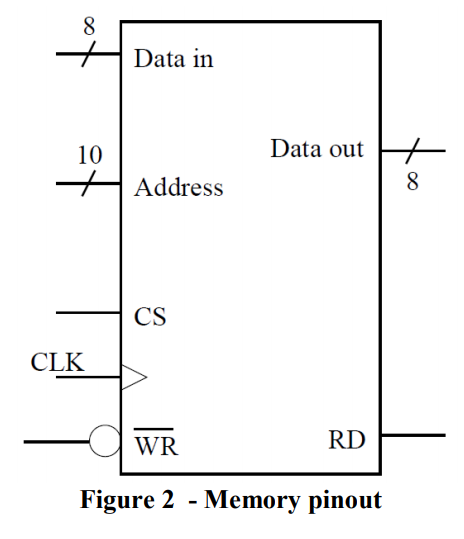
\includegraphics[scale = 0.7]{immagini/memory.png}
	\caption{ 1kByte memory }
\end{figure}

The memories store 1024 samples represented as 8 bit wide 2's complement values.
The writing operation is synchronous with the positive edge of the clock, while the reading is asynchronous. 

The samples must be stored in order, from address 0 to 1023.

Once the desired address is selected and the RD signal asserted, the output data are shown in the $ data out $ parallel output.

The figure below shows the testbench for the register file.
\newline\newline\newline
\begin{figure}[h]
	\centering
	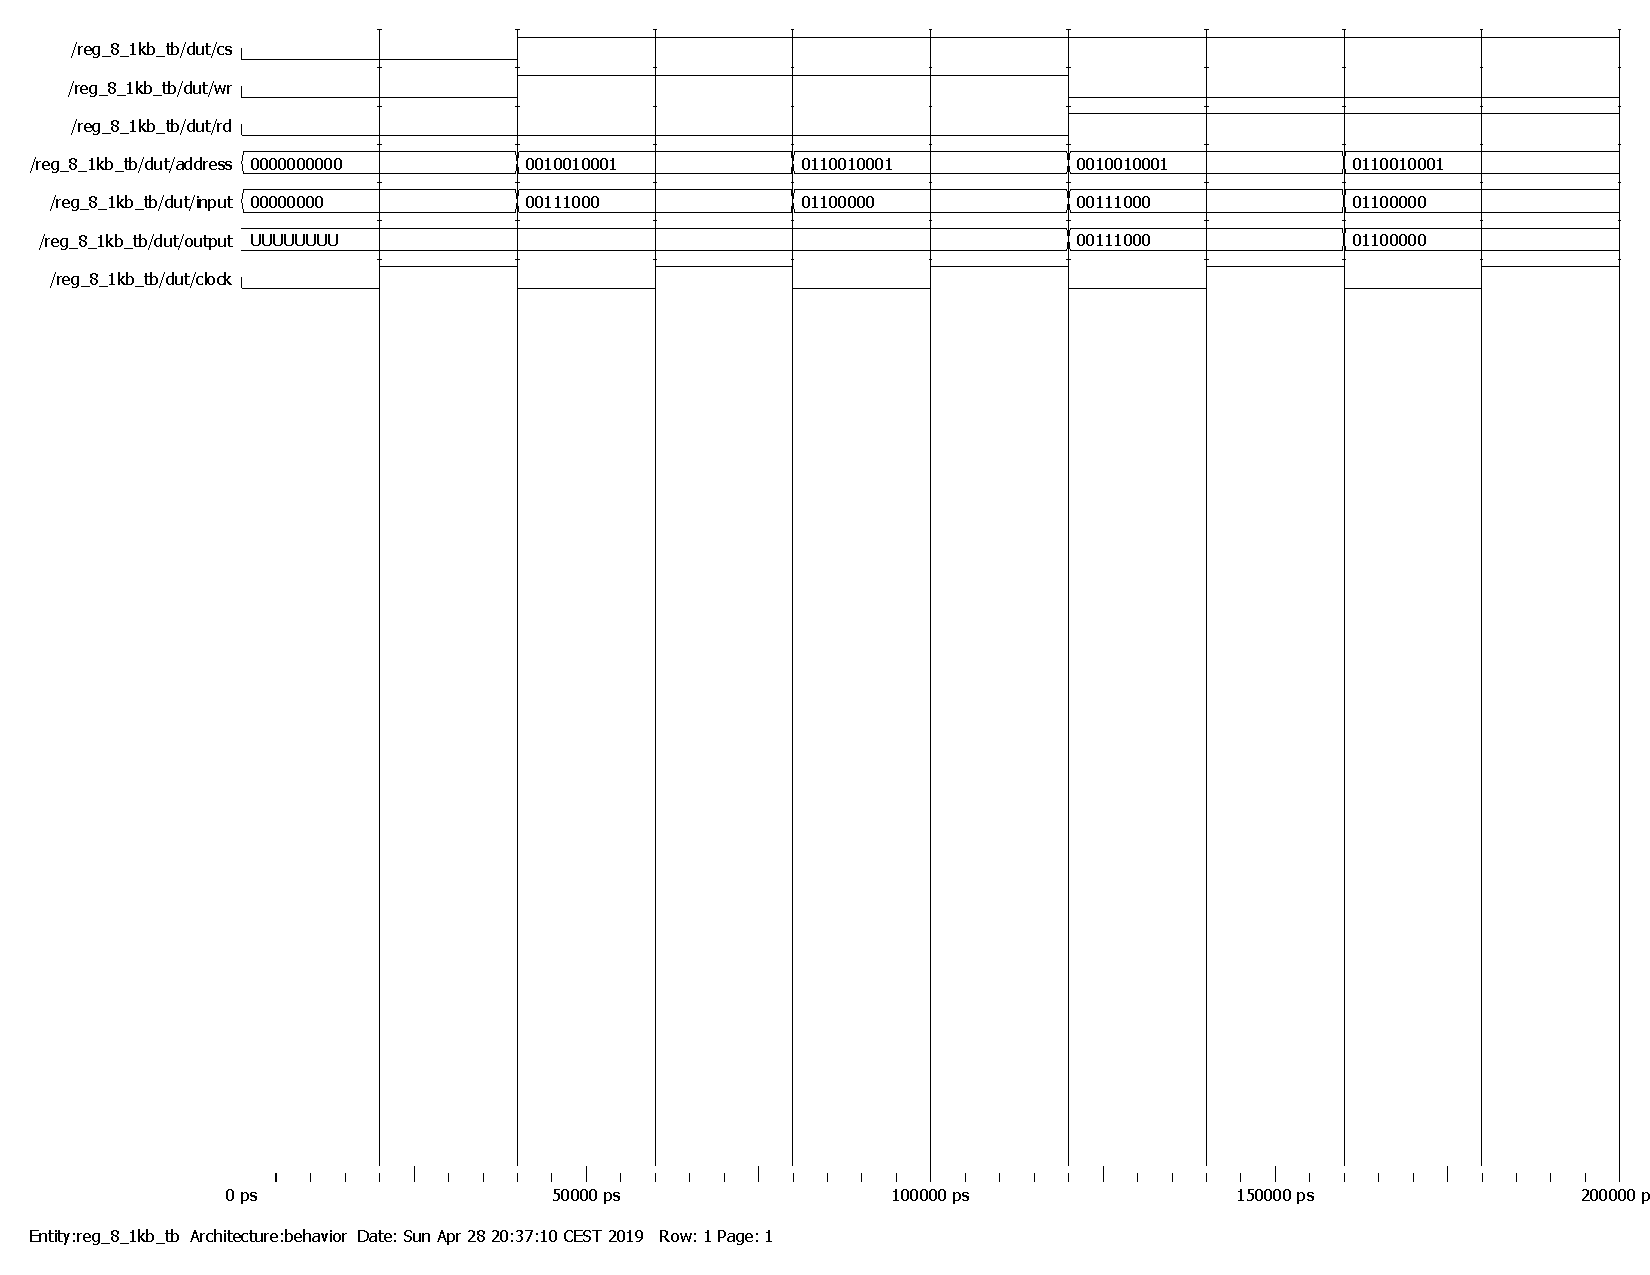
\includegraphics[scale = 0.55]{immagini/memory_tb.png}
	\caption{Memory testbench}
\end{figure}

\newpage
\subsection*{Shift registers and registers}

To be able to implement the already stated main equation, the circuit needs to perform 2s multiple multiplication and/or division.

The final implementation exploits the left and right shifting operations.

A 11 bit shift register has been implemented with parallel load and parallel output.

The $LOAD$ signal must be asserted to load the $parallel\;input$ data into the register, in a synchronous way with the positive edge of the clock.

The $SL$ and $SR$ commands permit the left or right shift of the internal memorized data.  
  

\begin{figure}[h]
	\centering
	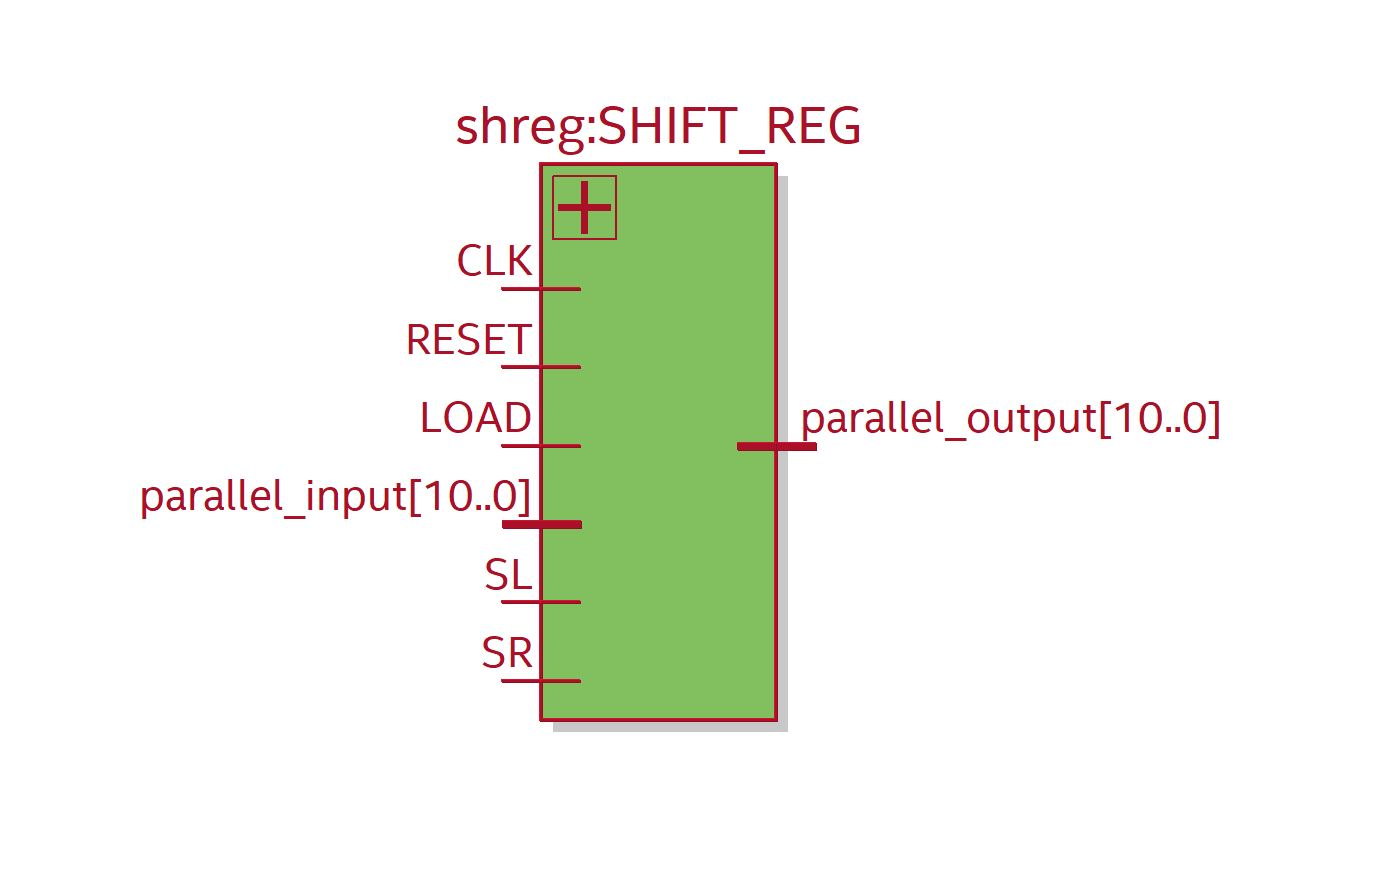
\includegraphics[scale = 0.6]{immagini/shreg.jpg}
	\caption{Shift register}
\end{figure}

The testbench for the 8-bit version is shown below:
 
\begin{figure}[h]
	\centering
	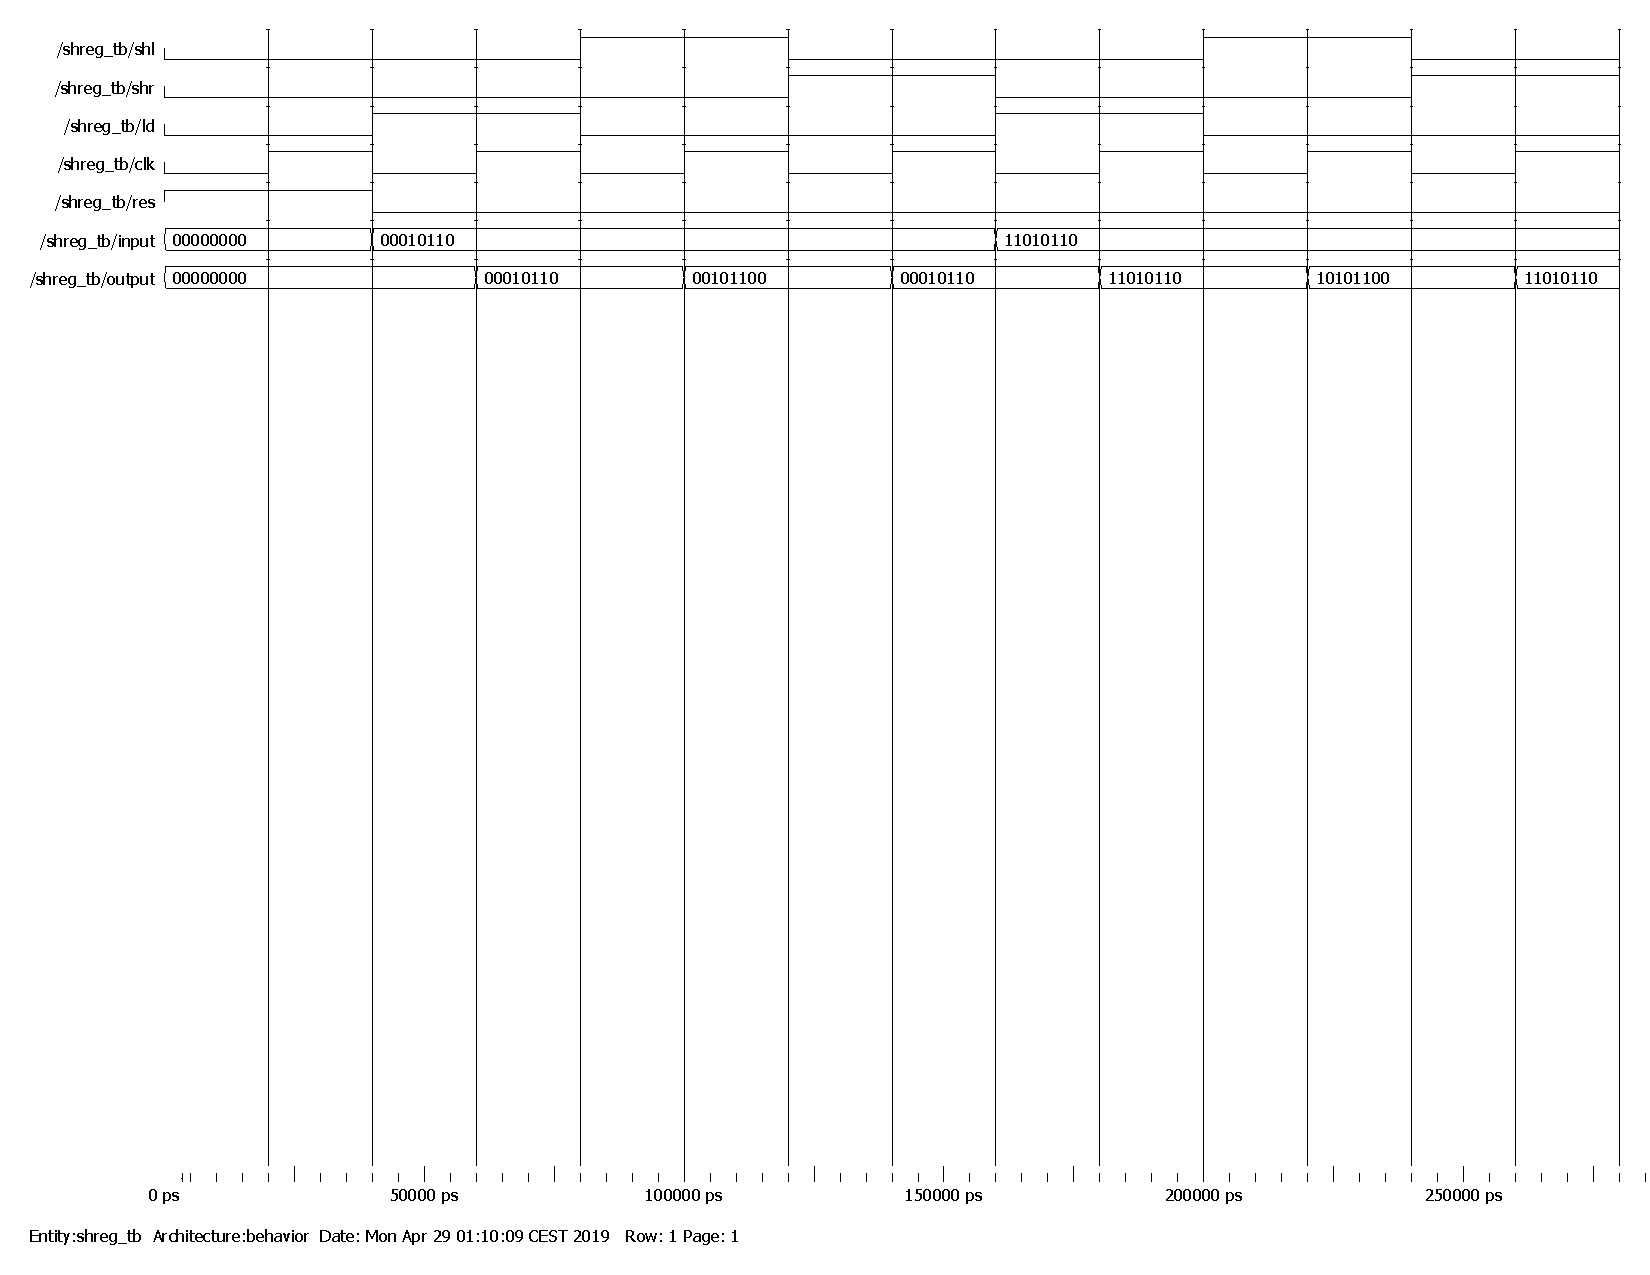
\includegraphics[scale = 0.55]{immagini/shift_reg_tb.png}
	\caption{Shift register test bench}
\end{figure}

\newpage

\subsection*{Adder}

An 11-bit of a classical adder has been implemented, allowed to perform additions and subtractions by means of the  $Cin$ signal.
\begin{figure}[h!]
	\centering
	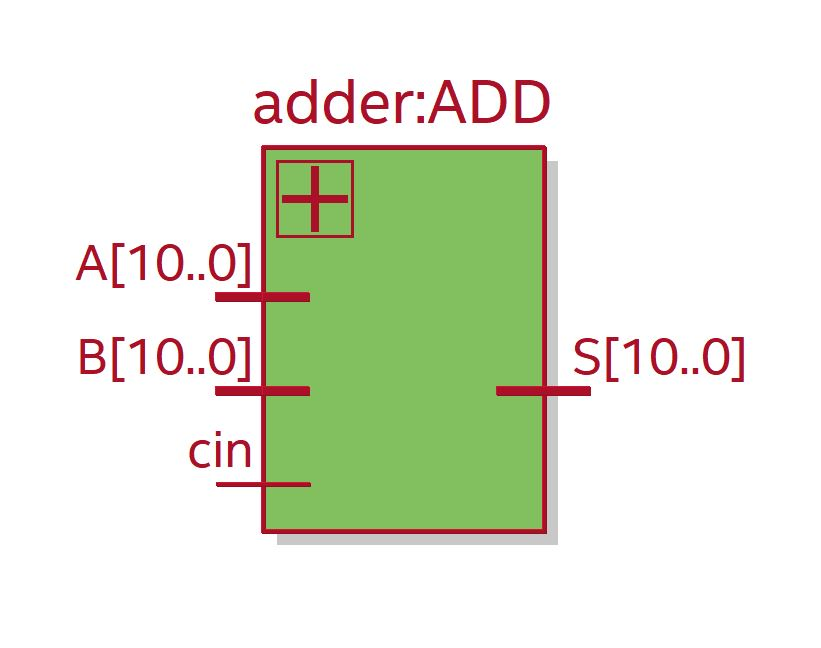
\includegraphics[scale = 0.65]{immagini/adder.jpg}
	\caption{Adder}
\end{figure}


Below is shown the test bench of the designed adder.


\begin{figure}[h]
	\centering
	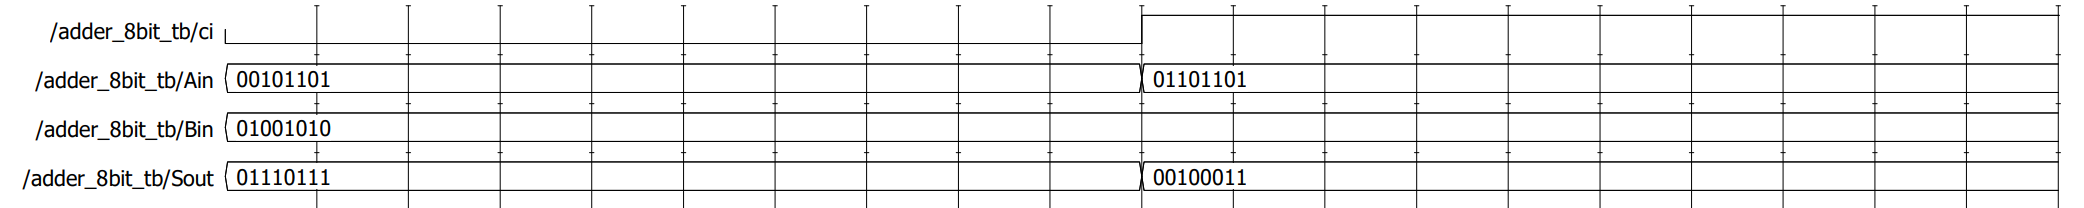
\includegraphics[scale = 0.55]{immagini/adder_tb.png}
	\caption{Adder test bench}
\end{figure}

\subsection*{Data converters}

Finally, since the circuit must be able to determine overflow/underflow and saturate the output if needed, it uses 2 blocks able to convert 8 bit signals to 11 bit and vice versa, as will be discussed in further sections. 

The simulated test bench are shown below: 

\begin{figure}[h!]
	\centering
	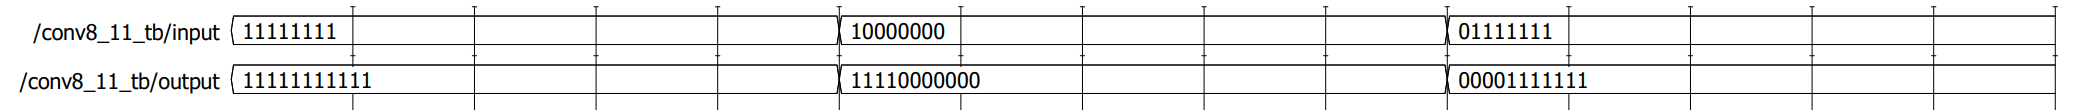
\includegraphics[scale = 0.47]{immagini/8_11_tb.png}
	\vspace{1mm}	
	\centering
	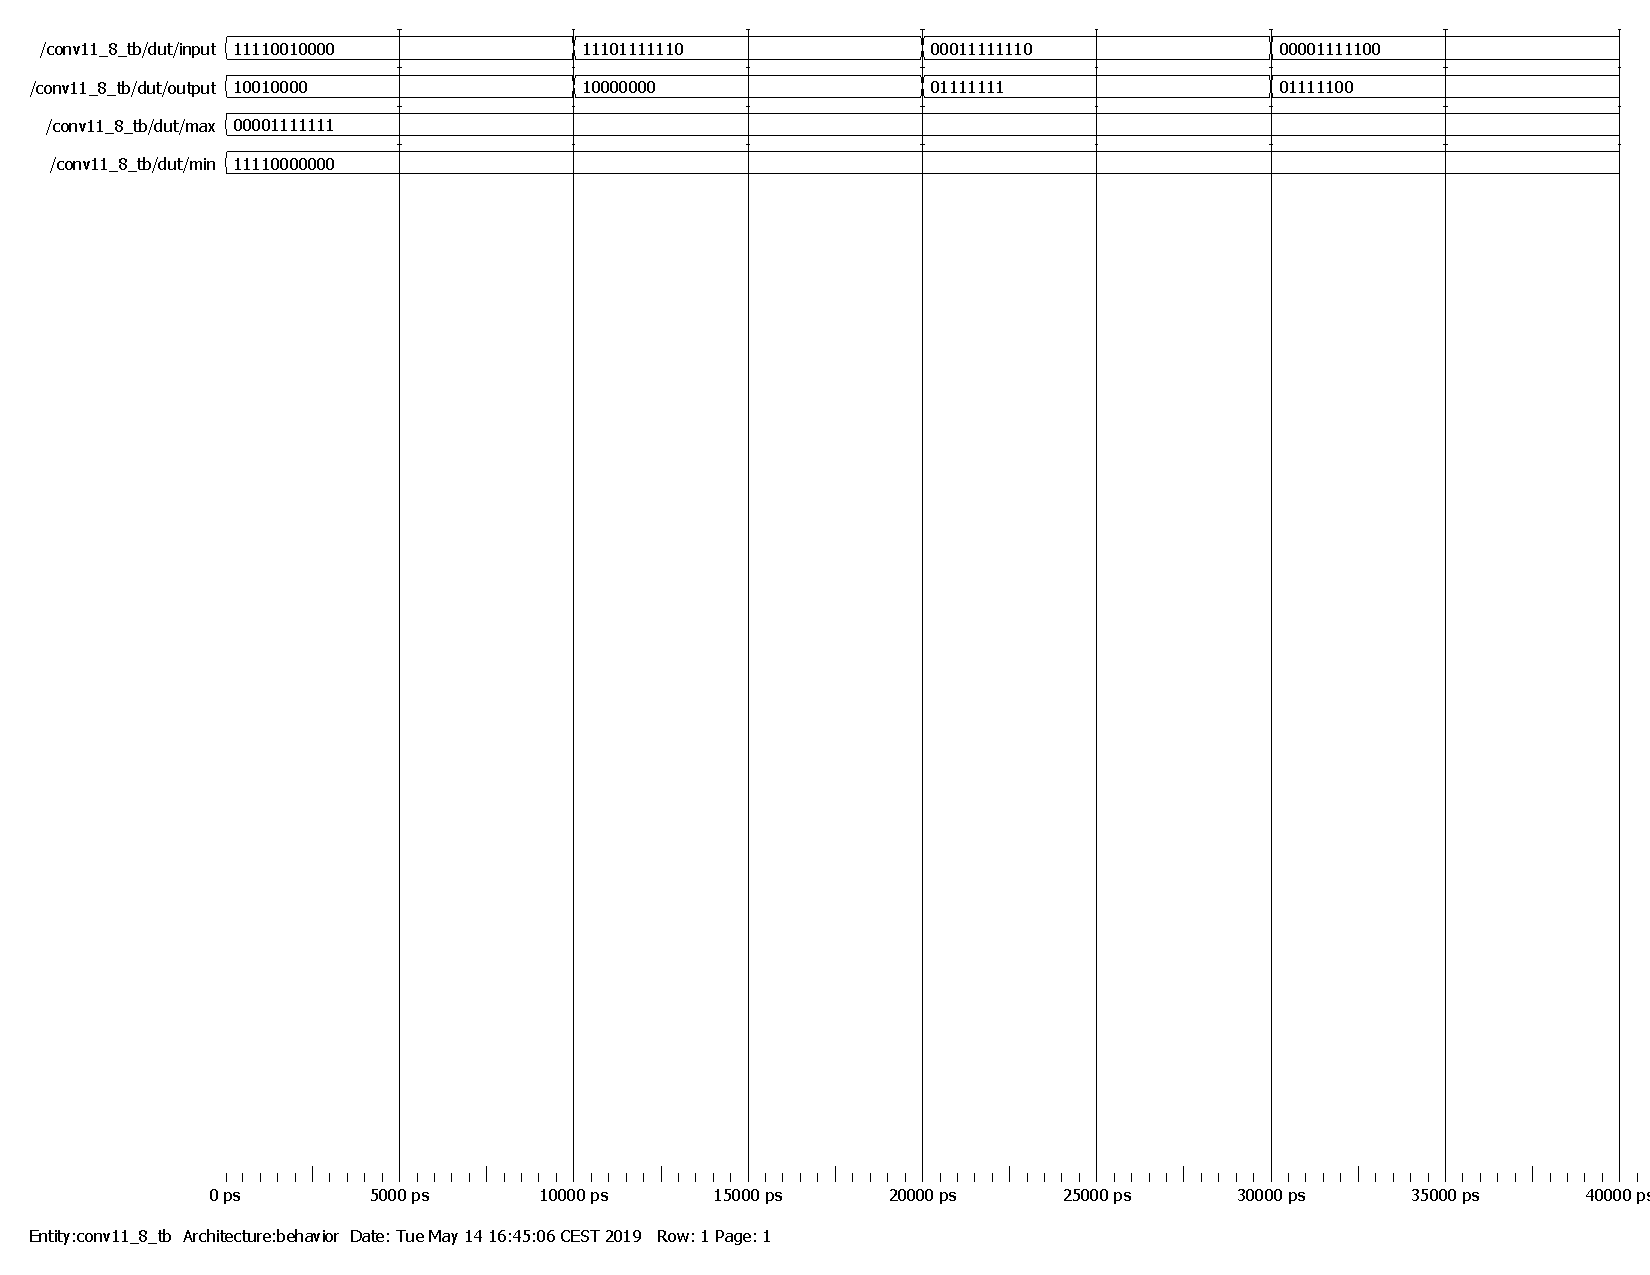
\includegraphics[scale = 0.47]{immagini/11_8_tb.png}
	\caption{8 to 11 bit converter; 11 to 8 bit converter}
\end{figure}
\newpage
\subsection*{Counter}
To be able to go through the various addresses an universal counter has also been implemented as shown: 
\begin{figure}[h!]
	\centering
	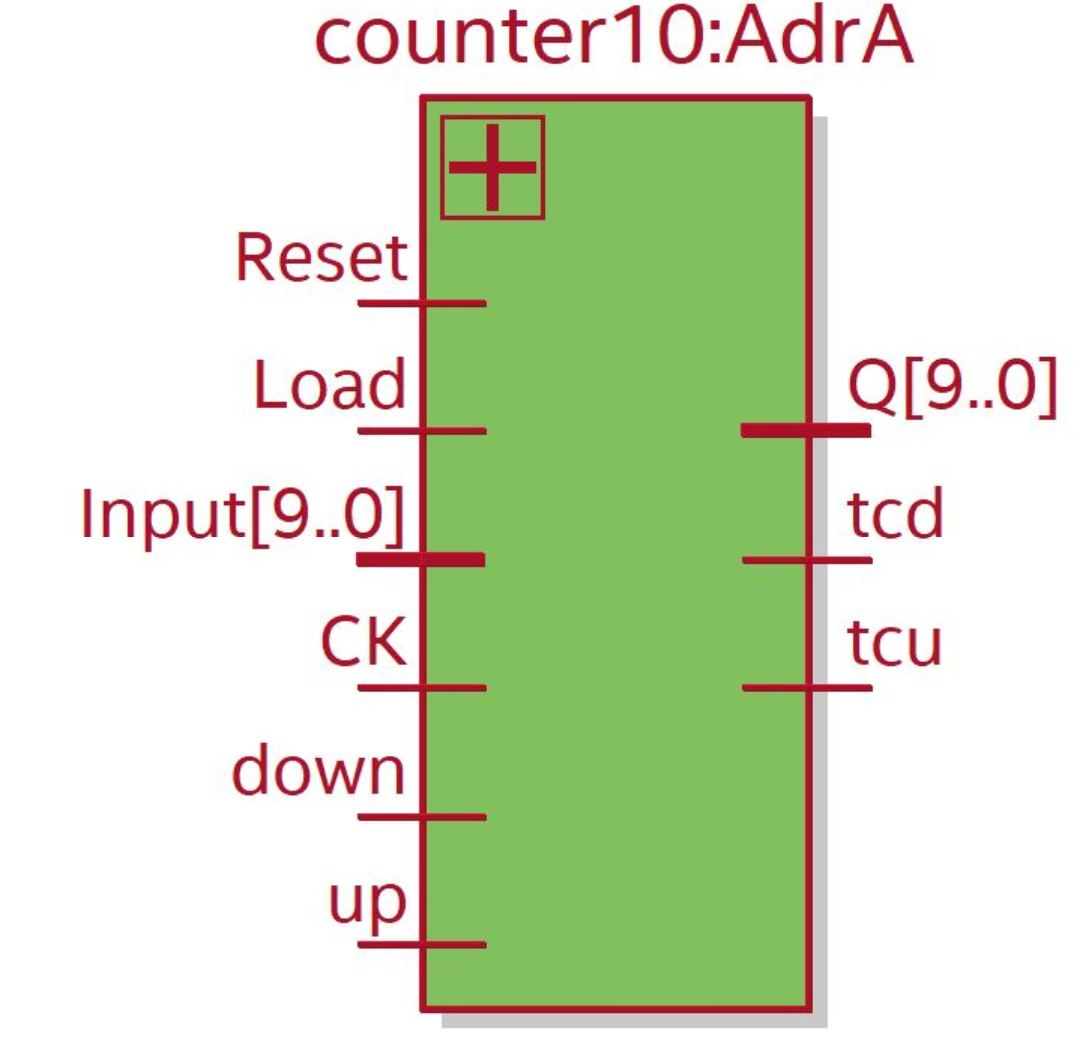
\includegraphics[scale = 0.47]{immagini/counter10.jpg}
	\caption{10 bit counter}
\end{figure}
The counter can count up or down. 
Furthermore, the output ports $tcd$ and $tcu$ have an high logical value when the counter reaches respectively its minimum or maximum possible value.

\begin{figure}[h]
	\centering
	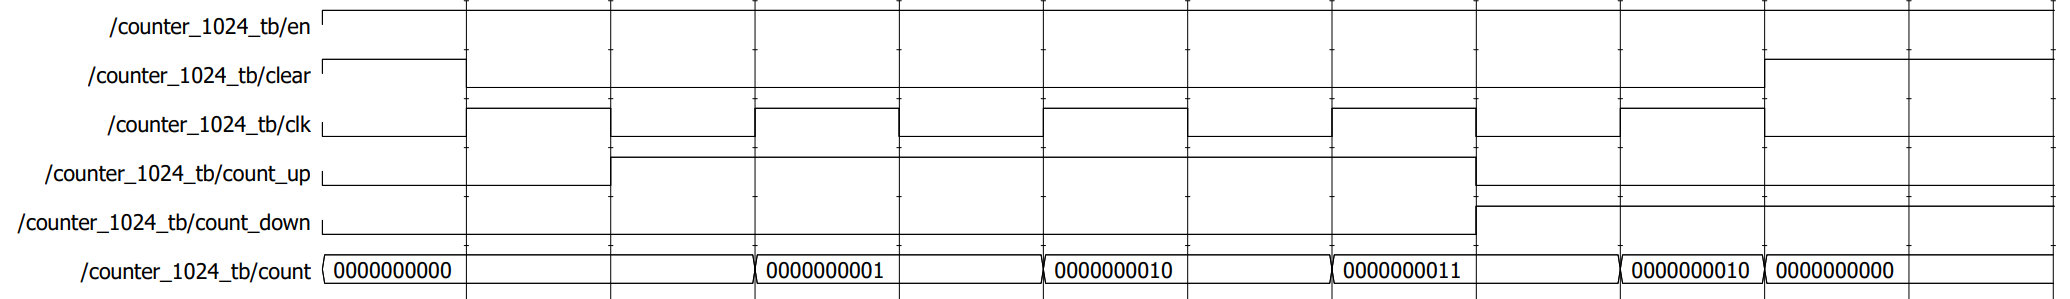
\includegraphics[scale = 0.47]{immagini/counter_tb.png}
	\caption{10 bit counter test bench}
\end{figure}
\newpage
\section*{Data path}
\begin{figure}[h]
	\centering
	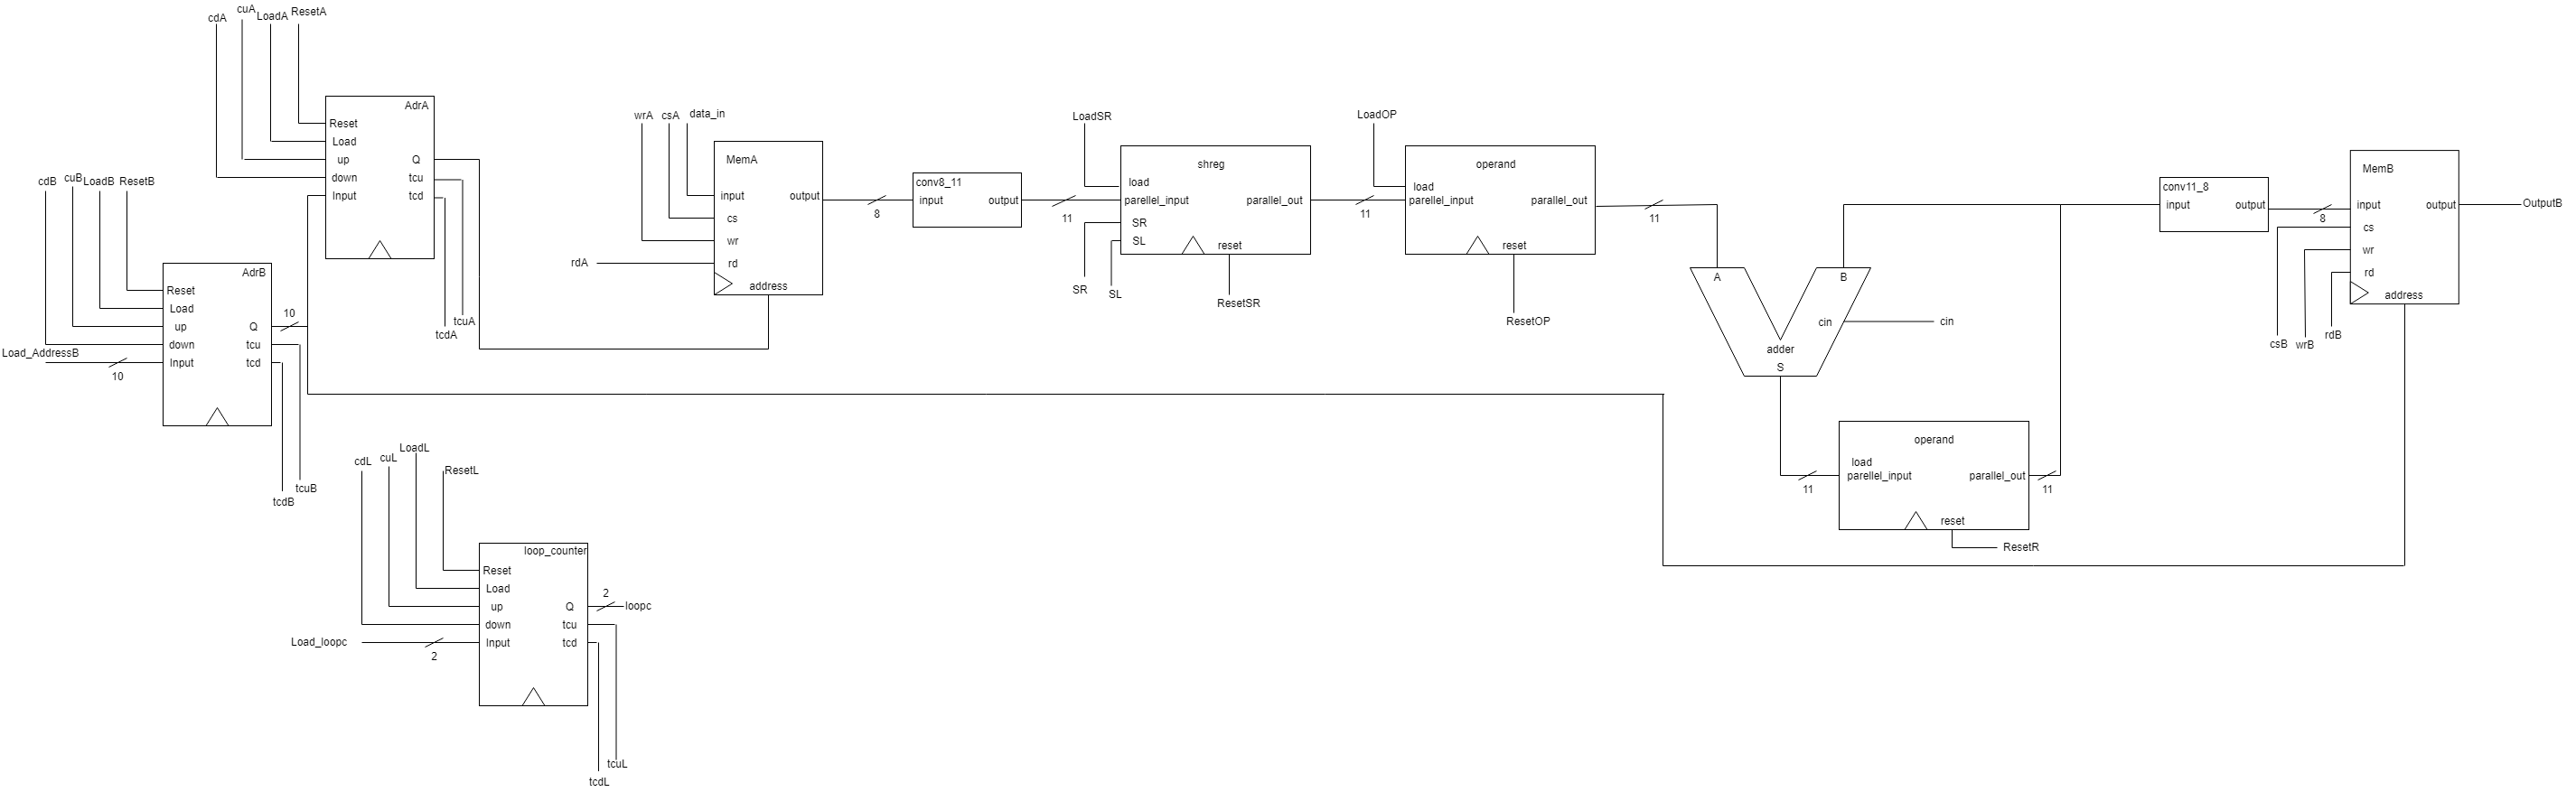
\includegraphics[scale = 0.17]{immagini/Datapath.png}
	\caption{Datapath}
\end{figure}
The data path of the filter has been designed with two primary goals: use the minimum number of components and simplify the control unit.\\
All the computations in the circuits are made on 11 bits (range: 1023 to -1024), because the biggest absolute value of $Y(n)$ is 864. \\
The computation of $Y(n)$ is performed in several steps:\\
1) an 8 bits number is read from Memory A converted to 11 bits and stored in the shift register\\
2)the shift register applies the proper division/multiplication factor\\
3)the multiplied/divided number is saved in the register $Operand$\\
4)in the register $Result$ is saved the content of the operation $Result +/- Operand$ with the proper sign\\
5)if the computation of $Y(n)$ is not complete we restart from step 1, if it is complete the value stored in $Result$ is converted to 8 bits and written in Memory B.\\

\section*{Control unit}
\begin{figure}[h]
	\centering
	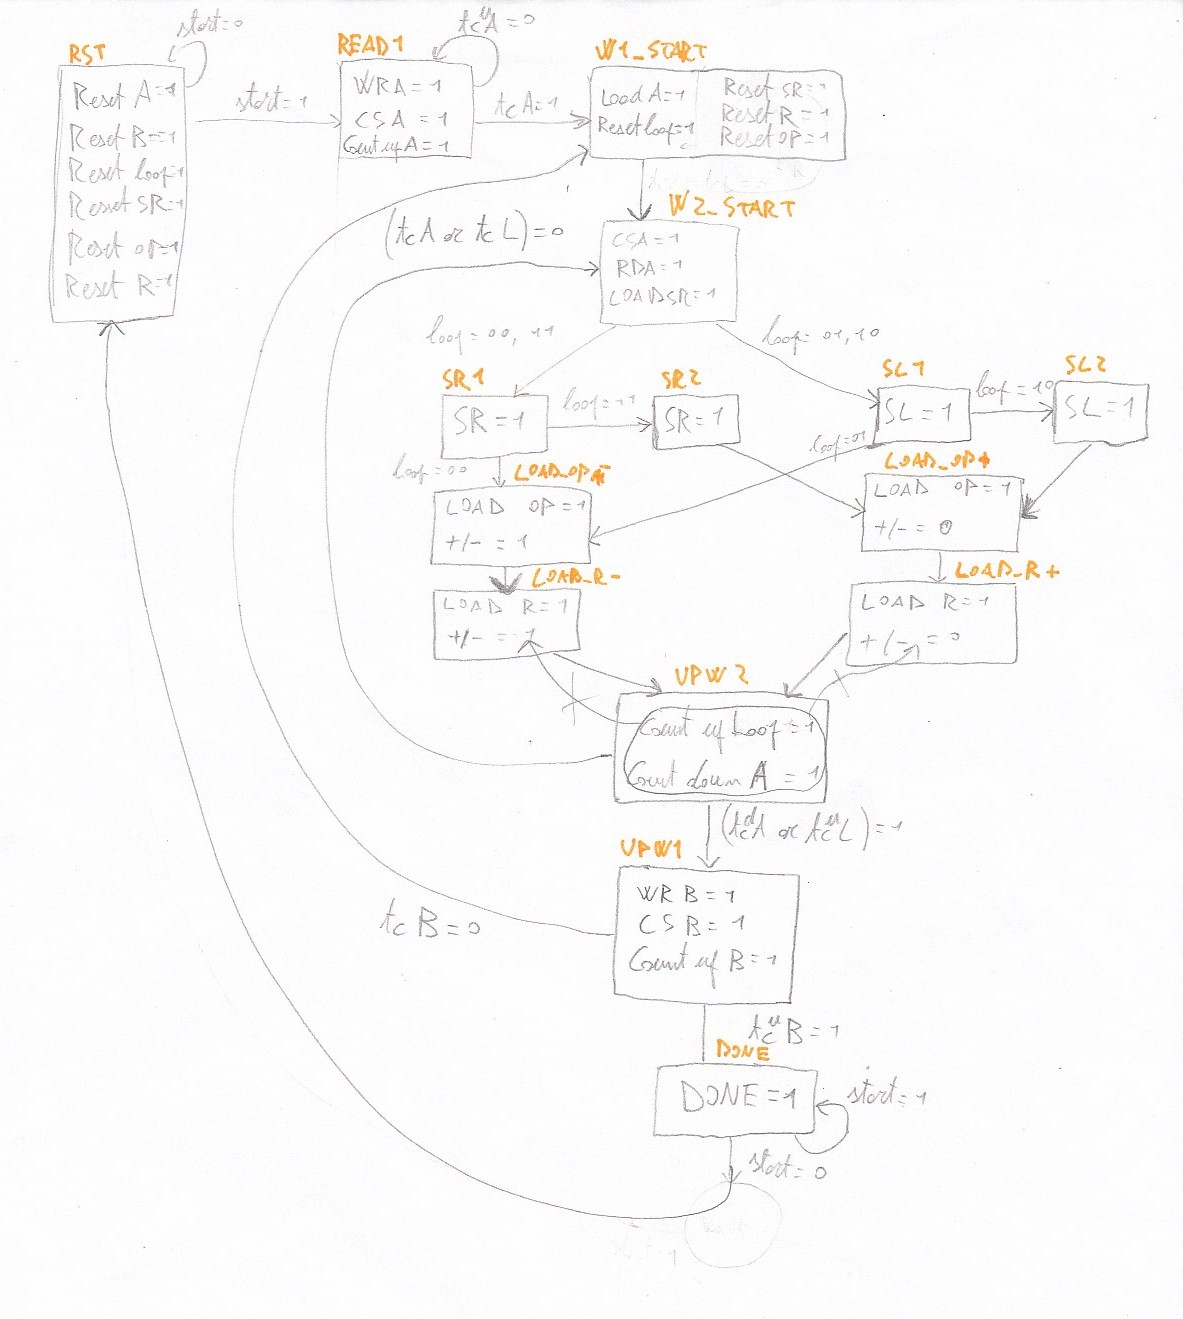
\includegraphics[scale = 0.85]{immagini/fsm.jpg}
	\caption{stade diagram of the control unit}
\end{figure}

The control unit has been implemented as a Moore finite state machine and is able to mange all the phases of the circuit: the acquisition and the computation.   \\
In the acquisition phase (state:$Read1$) the memory is selected and configured to write, the $counterA$ (which contains the address of A) is configured to count up. The cu remains in this state as long as the terminal counter up of $counterA$ remains to 0. \\

\begin{figure}[h]
	\centering
	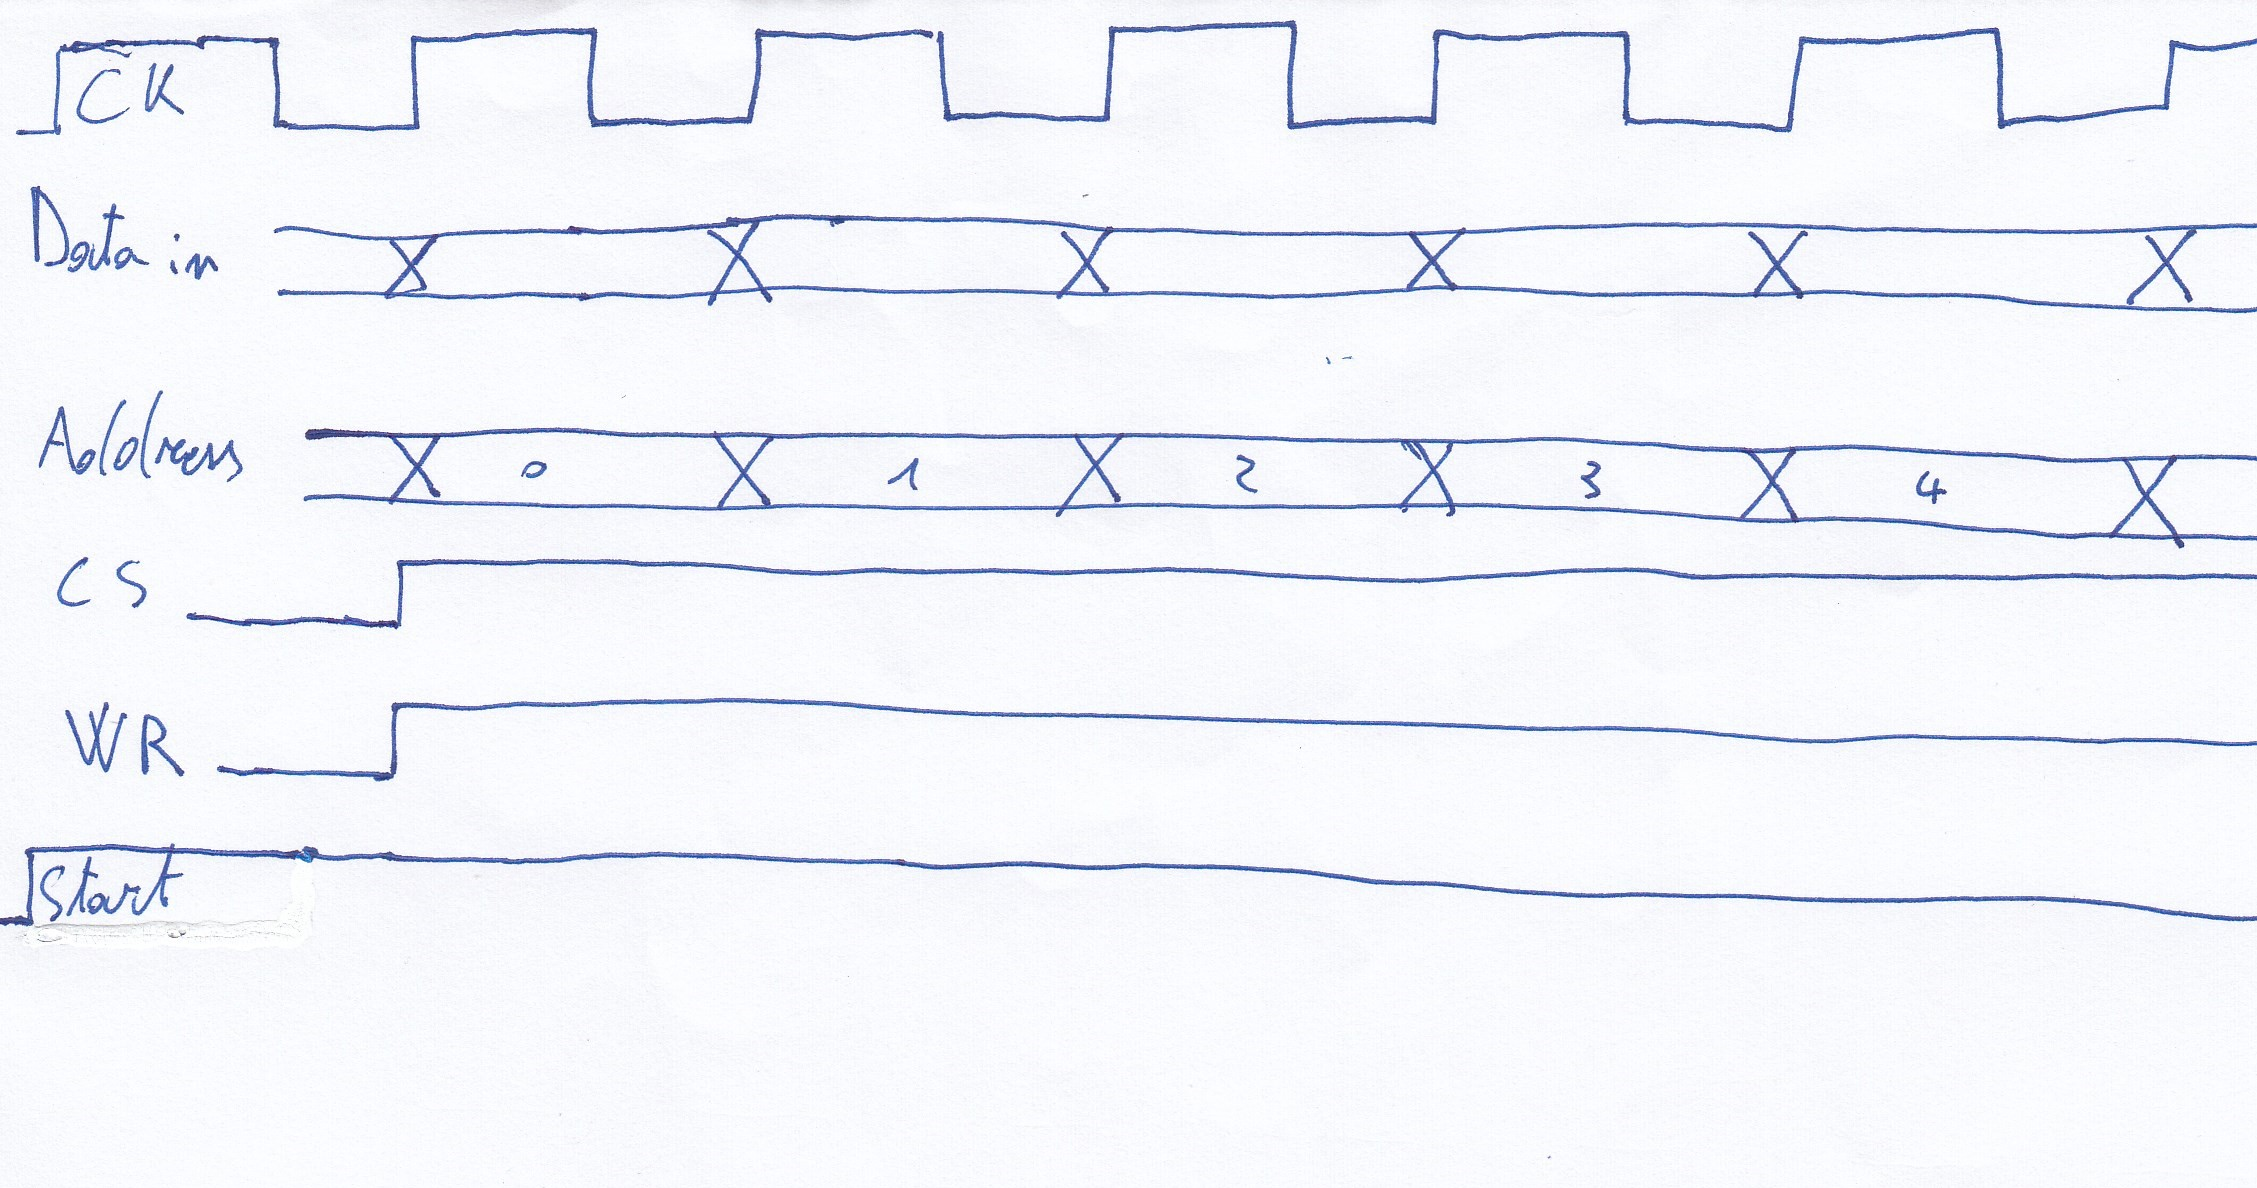
\includegraphics[scale = 0.55]{immagini/timing1.jpg}
	\caption{timing of read operations}
\end{figure}

The computation phase is done in two while loops: the first starts with $W1\_start$ and ends when the terminal counter up of $counterB$ is 1 that means that all $Y(n)$ have been computed and written in Memory B. The second loop starts with $W2\_starts$ and ends if the terminal counter down of $counterA$ is 1 therefore there are no valid addresses to retrieve the x(n-1/2/3) or if the terminal counter up of $loop$ is 1. The $loop$ counter is a 2 bit counter that is connected to the control unit and its value keeps track of the stage of the computation of $Y(n)$:\\
- when $loop=00$ $Y(n)=-0.5x(n)$ \\
- when $loop=01$ $Y(n)=-0.5x(n)-2x(n-1)$\\
- when $loop=01$ $Y(n)=-0.5x(n)-2x(n-1)+4x(n-2)$\\
- when $loop=11$ $Y(n)=-0.5x(n)-2x(n-1)+4x(n-2)+0.25x(n-3)$.\\

\begin{figure}[h]
	
	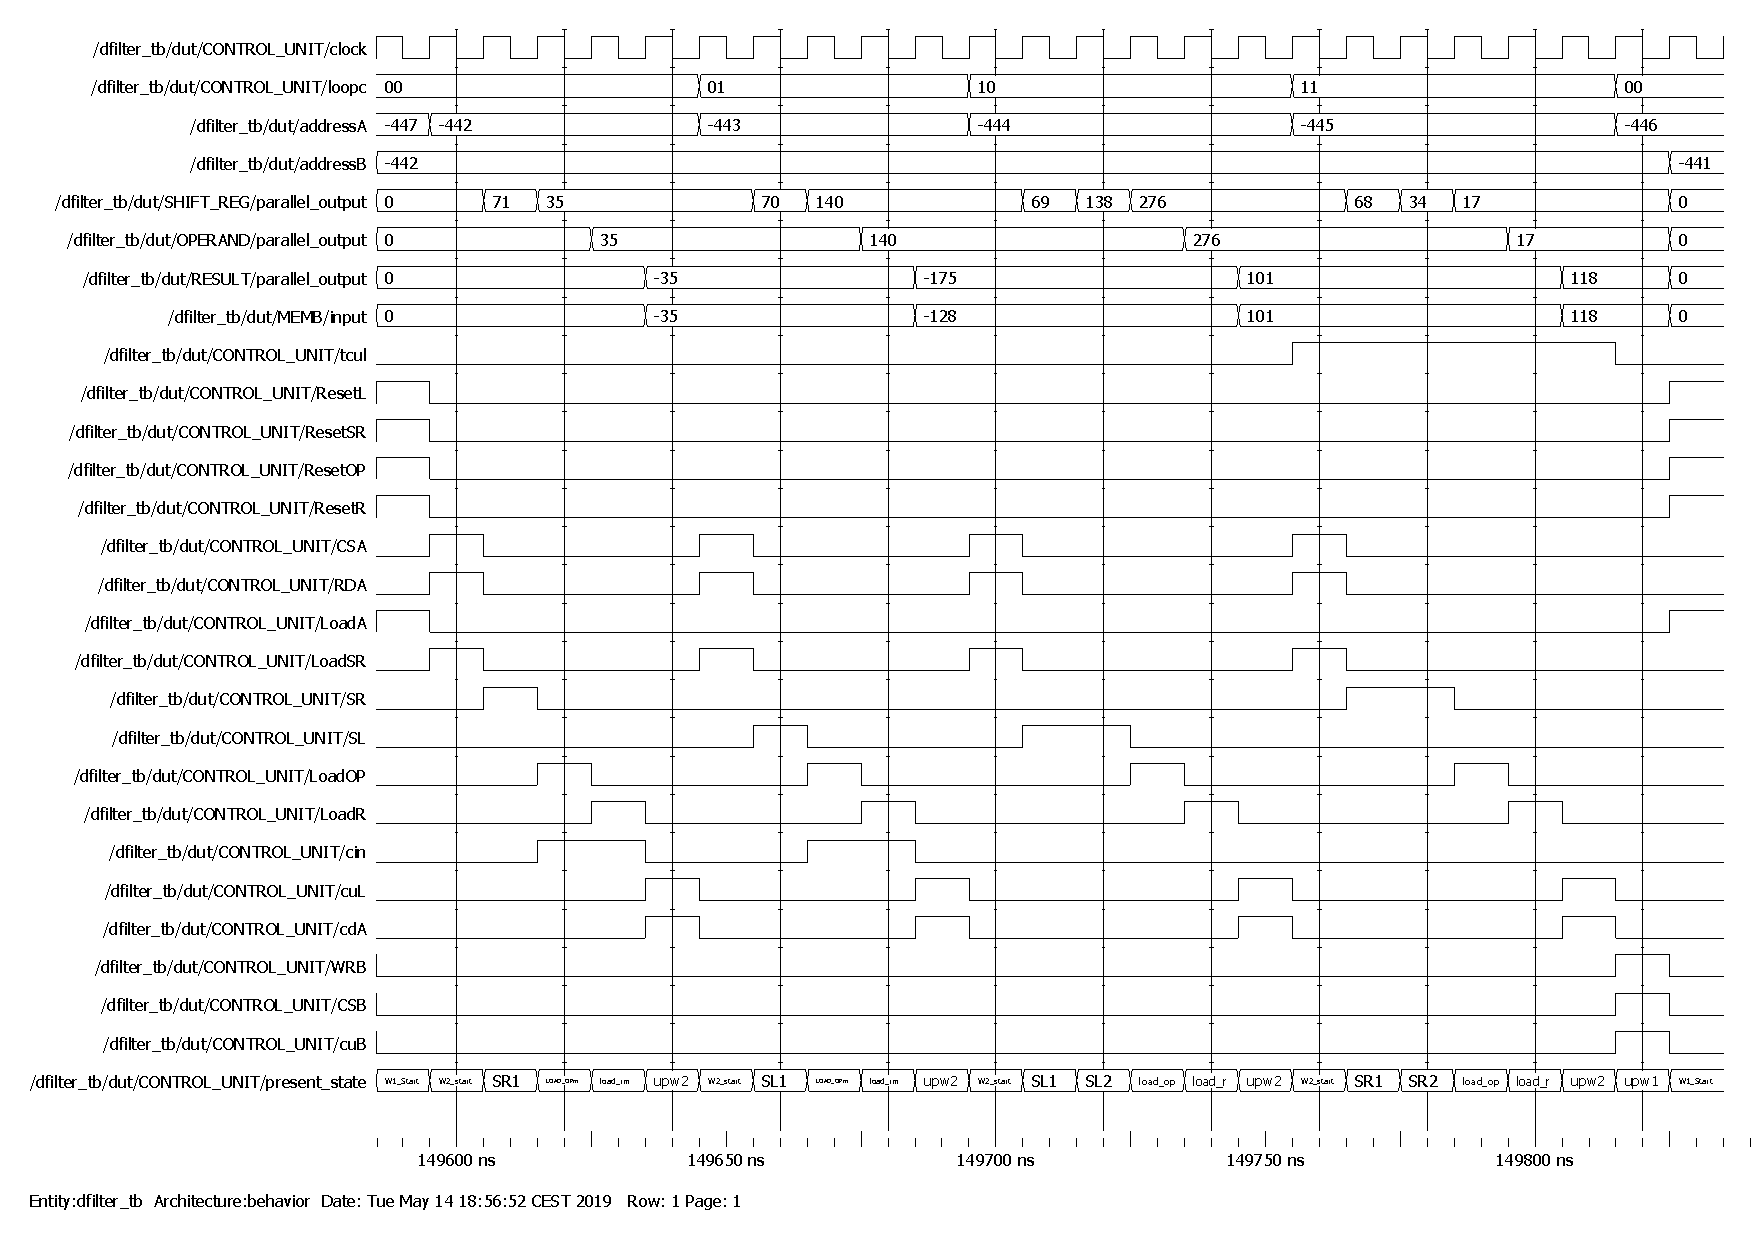
\includegraphics[scale = 0.59]{immagini/timing2.pdf}
	\caption{timing of a computation of Y(n)}
\end{figure}



\section*{Testbench}
In the file $dfilter\_tb$ there is a simple testbench where is generated a clock and given to the circuit the input data. The input data have been generated with a counter that counts from 0 to 1023 in unsigned 8 bits numbers. \\
With the help of Modelsym we are able to make to simulate the circuit until it finishes its computations and asserts the done output, than go to the memory panel and save as a file the contents of the memories A and B in binary form in two distinct files A.mem and B.mem, where we removed the first part of comment generated from Modelsym. \\
Using a custom Matlab script we are able to read both the files and perform in Matlab the same operations of the circuit using as input data the data read from A.mem and than compare the results. 

\section*{Attached files}
In addition to the VHDL sources, there are also: the matlab script and samples A.mem and B.mem filese to test the circuit, the pseudcode of the algorithm, the ASM chart of the CU, the ASM chart of the algorithm, the datapath, the state diagram of the CU and a waveform sample from modelsym.
\end{document}




